Another implementation of the scan is with the algorithm developed by Blelloch \cite{BlellochTR90}. The Blelloch scan is based on a balanced tree, consisting of two phases, the up-sweep phase and the down-sweep phase. A visual representation of the Blelloch scan is seen in \cref{fig:scan_blelloch}. 

\begin{figure}[ht]
	\centering
	\fbox{
		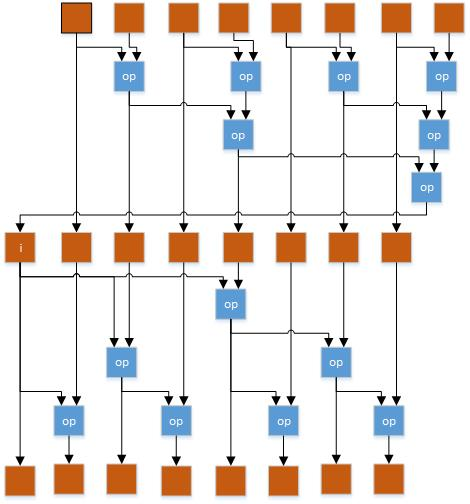
\includegraphics[width=0.4\textwidth]{figs/algorithm/scan_blelloch.jpg}}
	\caption{TBD}
	\label{fig:scan_blelloch}
\end{figure}

The first phase, the up-sweep, is a reduction as described in \cref{sec:al_reduction}. The reduction will only produce the entire sum and partial tree summations, this is why the down-sweep is necessary. The down-sweep start with the identity element and start from the root and goes to the leaves, opposite of the reduction mechanics, as seen in \cref{fig:scan_blelloch}. The Blelloch scan in its representation is an exclusive scan, but can be made inclusive scan through array shifting, or by implementation as seen in \cref{fig:scan_inclusive}.

\begin{figure}[ht]
	\centering
	\fbox{
		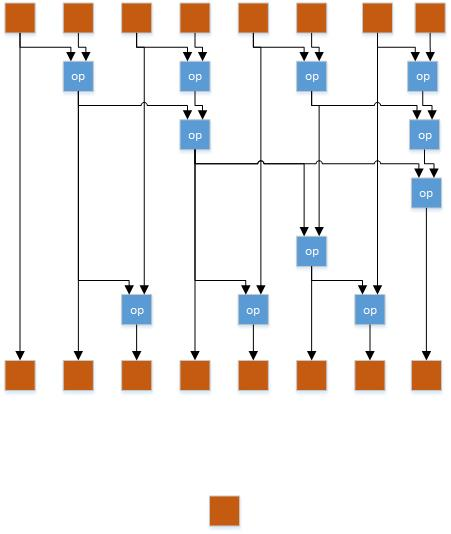
\includegraphics[width=0.4\textwidth]{figs/algorithm/scan_inclusive_parallel.jpg}}
	\caption{TBD}
	\label{fig:scan_inclusive}
\end{figure}

The up-sweep and down-sweep in their inclusive form is equal in terms of step and work complexity. The up-sweep is a reduction, with O(n) work and O(log n) steps, meaning the Blelloch scan has O(2 n) work and O(2 log n) step complexity. The Blelloch scan is step efficient compared with the serial implementation, but not as step efficient as the Hillis/Steele scan. The Blelloch scan is on the other hand a lot more work efficient than the Hillis/Steele. In a case where there are more array elements than processors the Blelloch scan would prove faster than the Hillis/Steele. It is therefore application specific which scan should be used.

[Overvej kode example].